%------------------------------------------------
\section{Стохастическое охлаждение}

\begin{frame}
	\frametitle{Стохастическое охлаждение}
	\par Метод уменьшения эмиттанса пучка за счёт использования системы с отрицательной обратной связь.
	\newline
	\par С ростом интенсивности пучка, эффективность СО падает.
	\begin{figure}[t]
		\centering
		
\includegraphics[width=9cm]{stochastic}
		\label{fig:stochastic}
	\end{figure}
\end{frame}
%------------------------------------------------
\begin{frame}
	\frametitle{Комбинированная структура}
	\begin{columns}[t]
		\begin{column}{0.4\textwidth}
			\begin{itemize}
				\item Применяется для увеличения эффективности стохастического охлаждения.
				\item Критическая энергия выше энергии эксперимента.
				\item Требуется сильная модуляция.
				\item Оптимизация ДА -- секступольная коррекция.
			\end{itemize}
		\end{column}
		\begin{column}{0.6\textwidth}
			\begin{figure}[t]
				\centering
				
\includegraphics[width=10cm]{combined}
				\label{fig:combined}
			\end{figure}
		\end{column}
	\end{columns}	
\end{frame}
%------------------------------------------------
\begin{frame}
	\frametitle{Аналитическая оценка}
	\centering
	\par Светимость $L = 2 \times 10^{32} \text{ см}^{-2} \cdot \text{с}^{-1}$
	\begin{figure}[ht]
		\centering
		\begin{minipage}{0.45\textwidth}
			\centering
			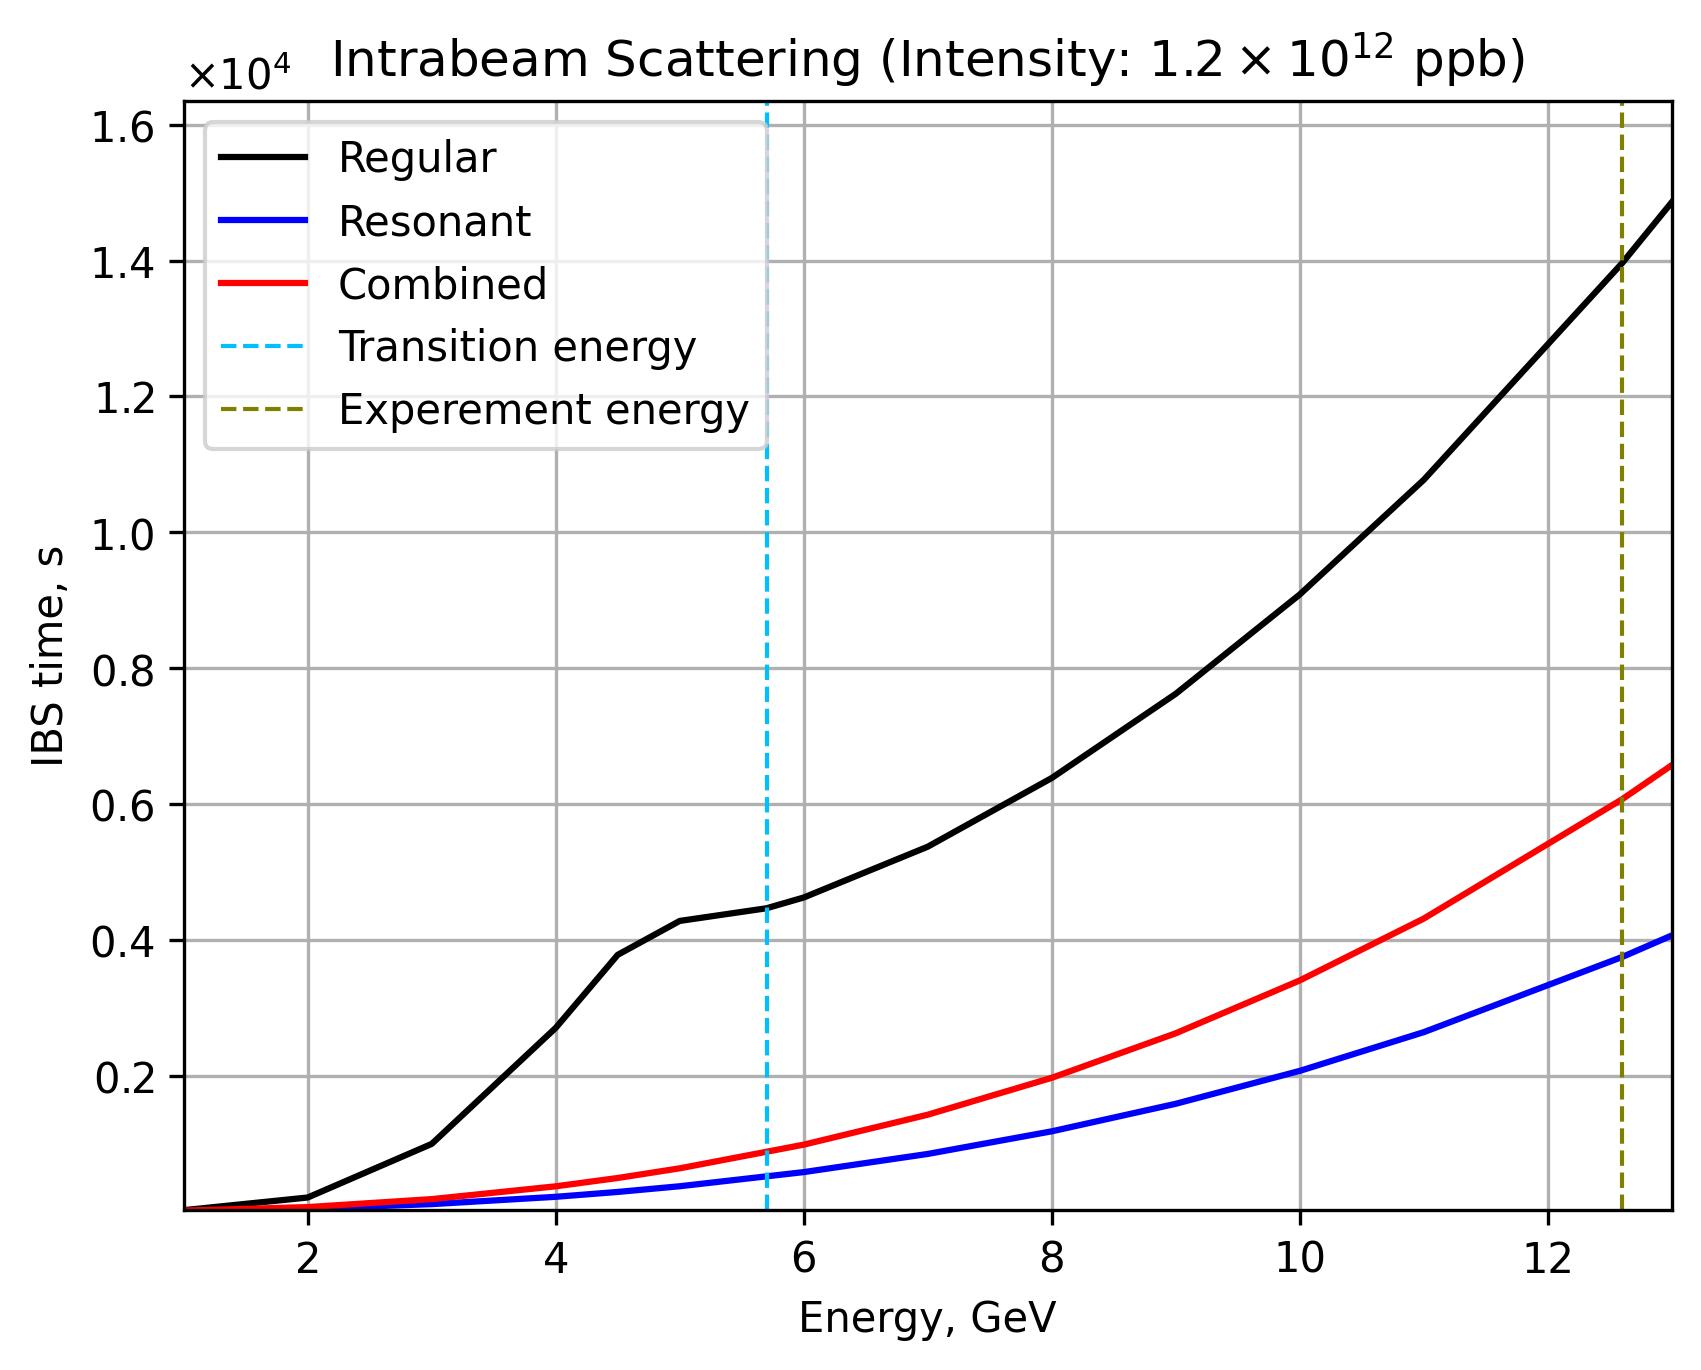
\includegraphics[width=\linewidth]{images/IBS_1_2e+12_png}
			\label{fig:ibs12e12png}
		\end{minipage}
		\hfill
		\begin{minipage}{0.45\textwidth}
			\centering
			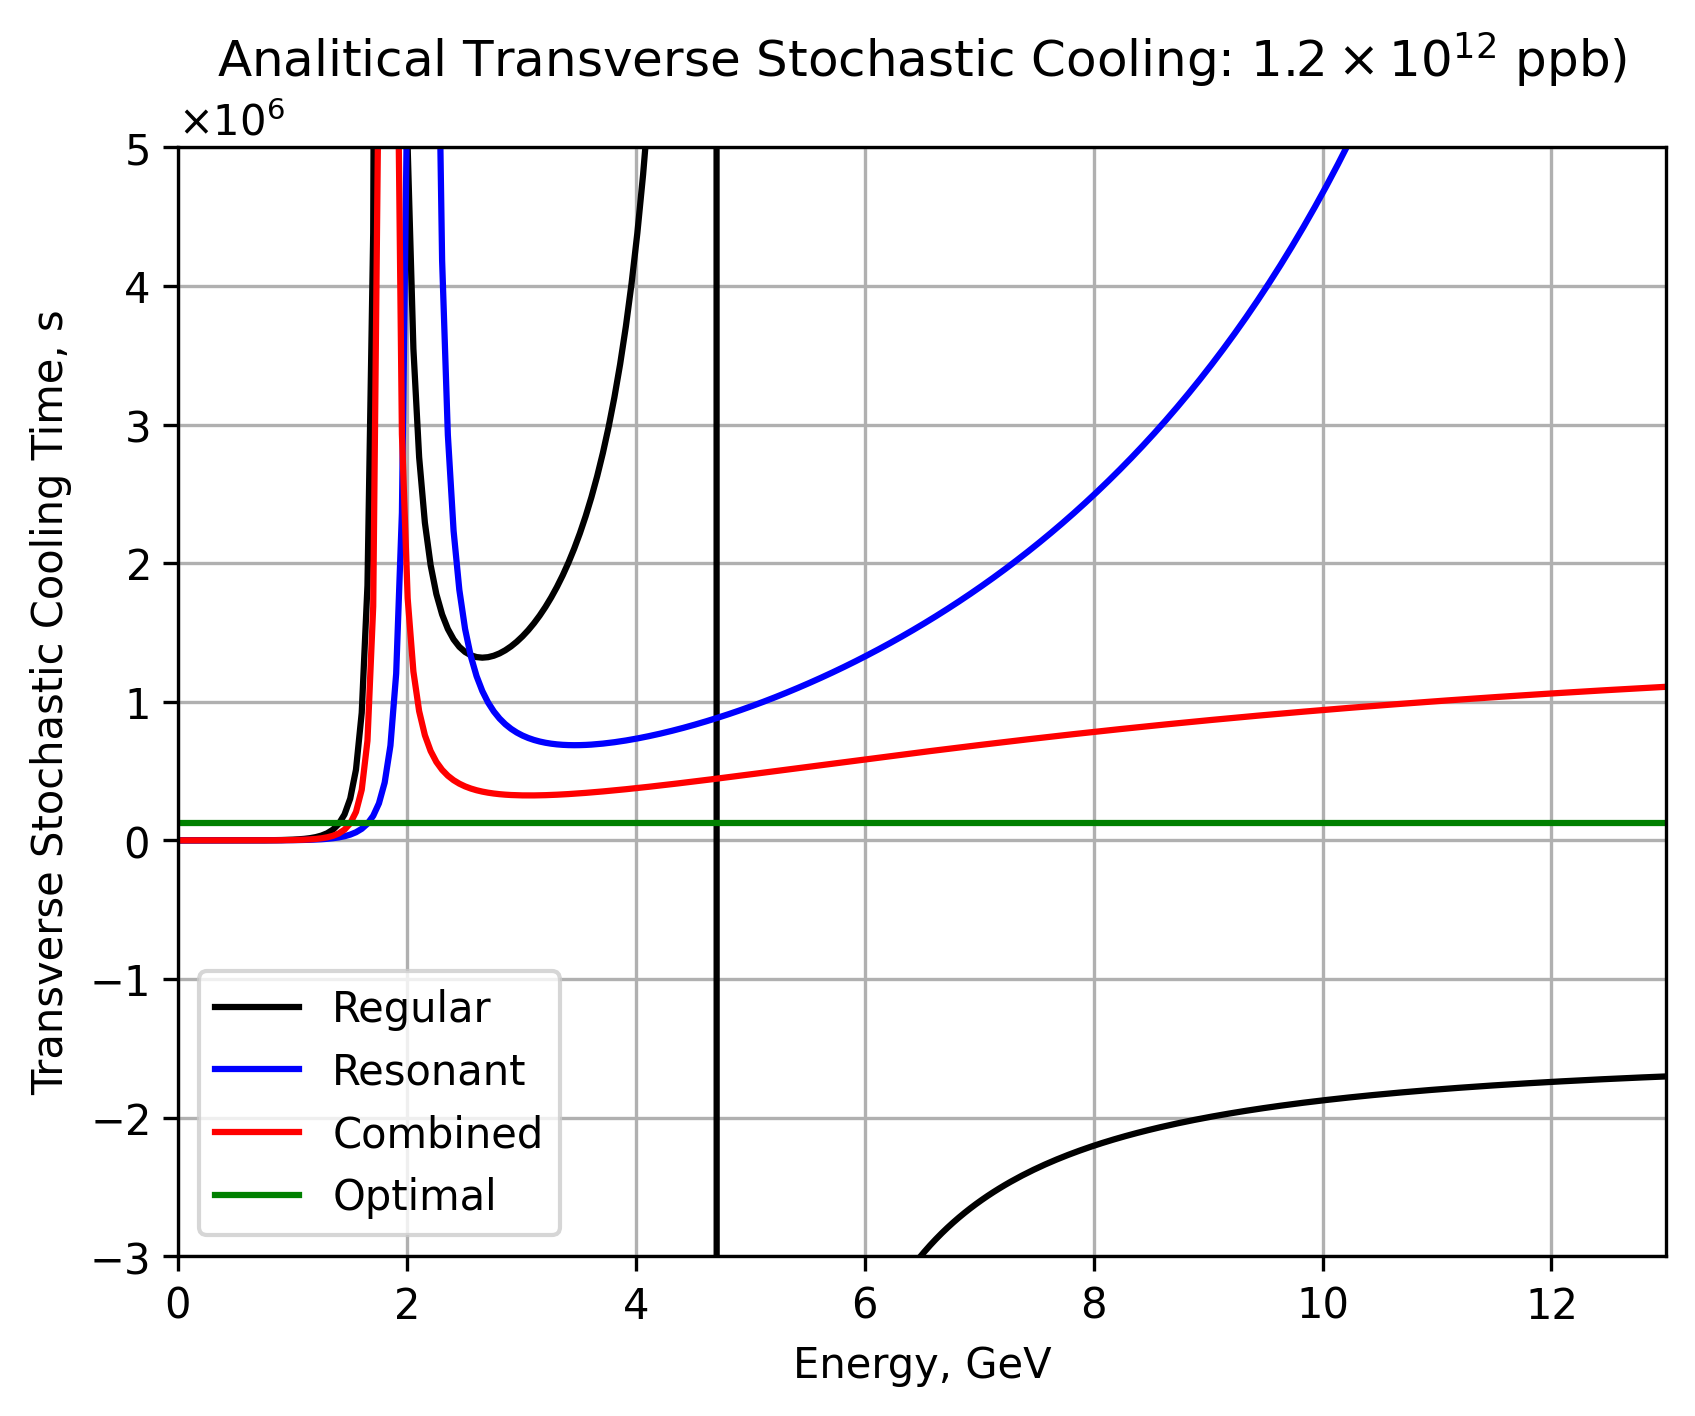
\includegraphics[width=\linewidth]{images/SC_1_2e+12_png}
			\label{fig:sc12e12png}
		\end{minipage}
	\end{figure}
\end{frame}
%------------------------------------------------
\begin{frame}
	\frametitle{Аналитическая оценка для меньшей интенсивности}
	\begin{figure}[ht]
		\centering
		\begin{minipage}{0.45\textwidth}
			\centering
			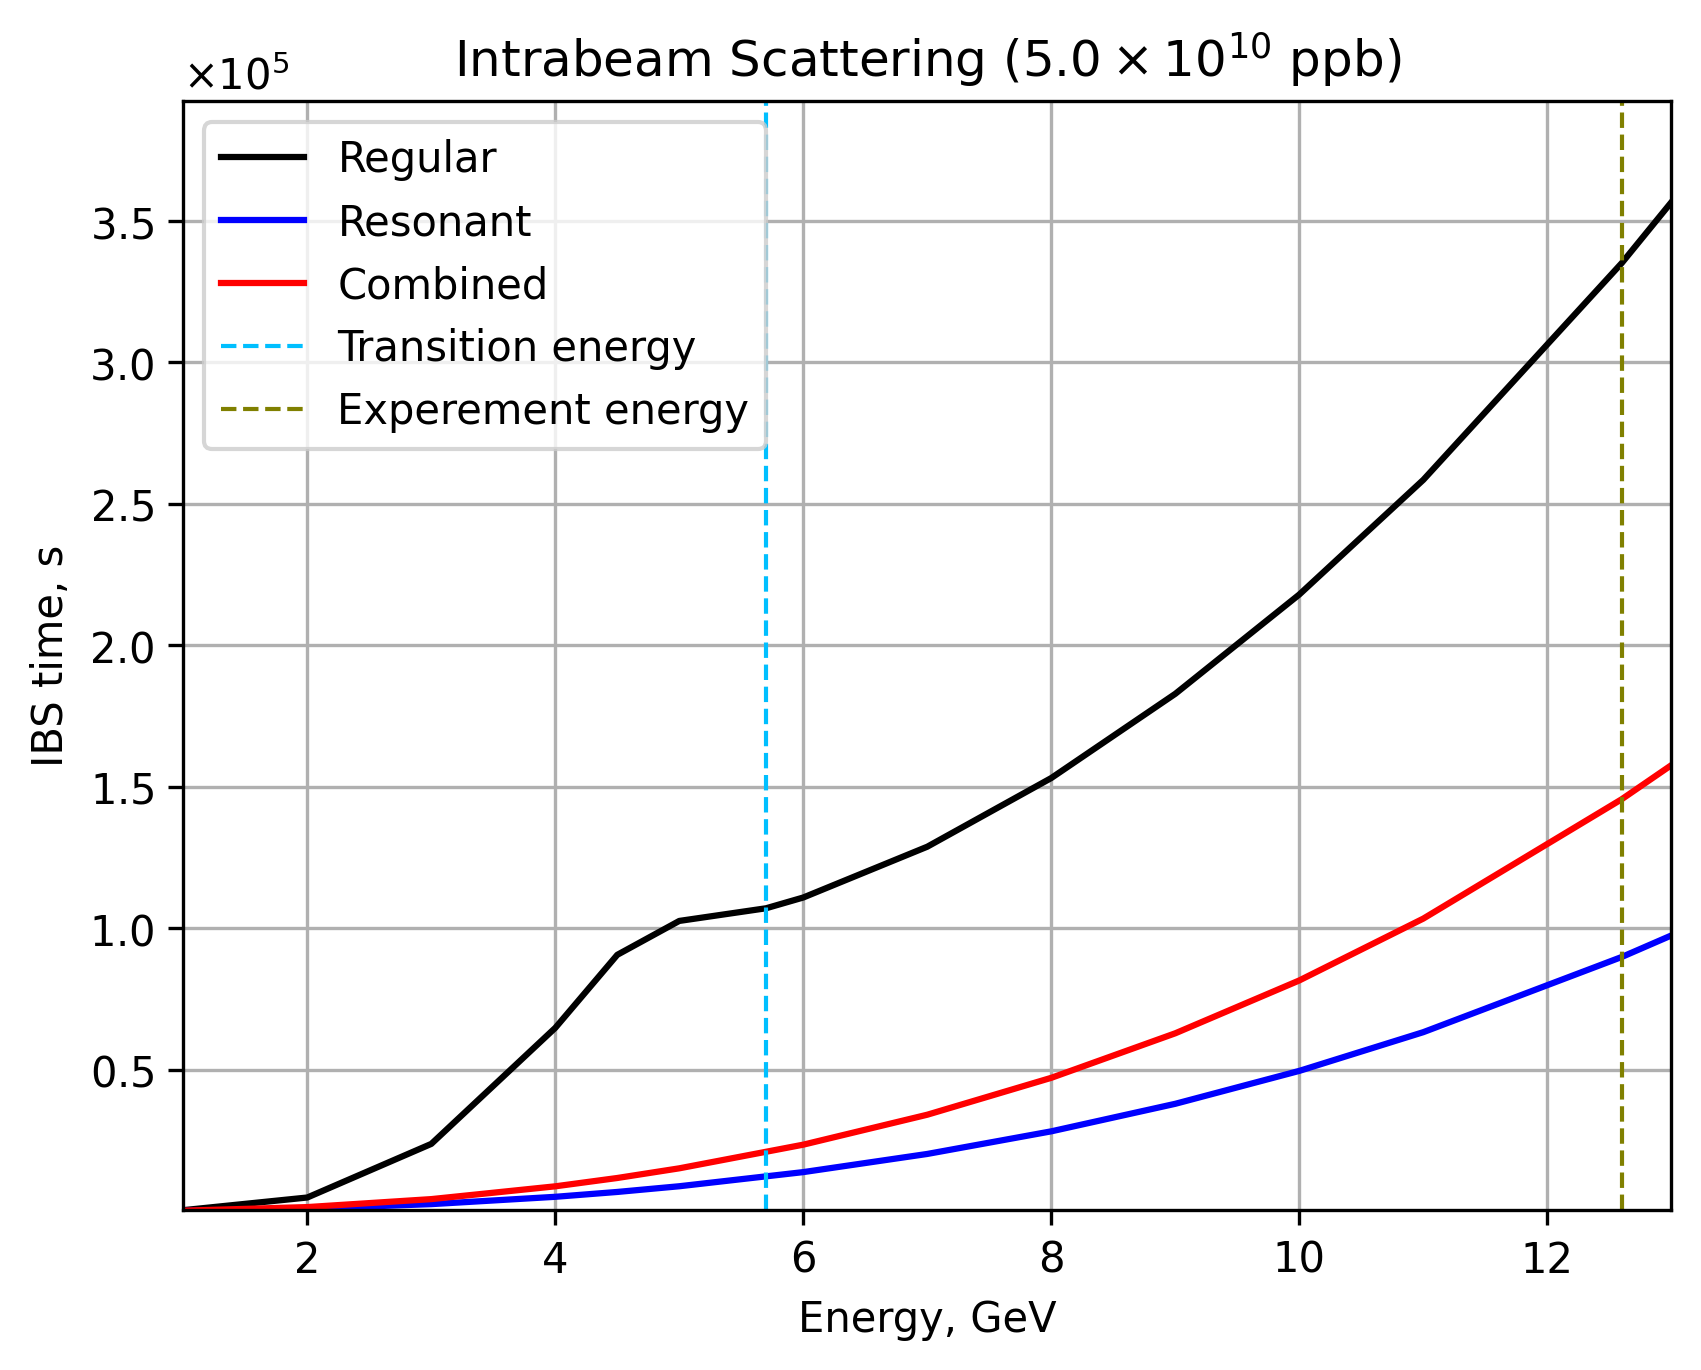
\includegraphics[width=\linewidth]{images/IBS_5_0e+10_png}
			\label{fig:ibs10e11png}
		\end{minipage}
		\hfill
		\begin{minipage}{0.45\textwidth}
			\centering
			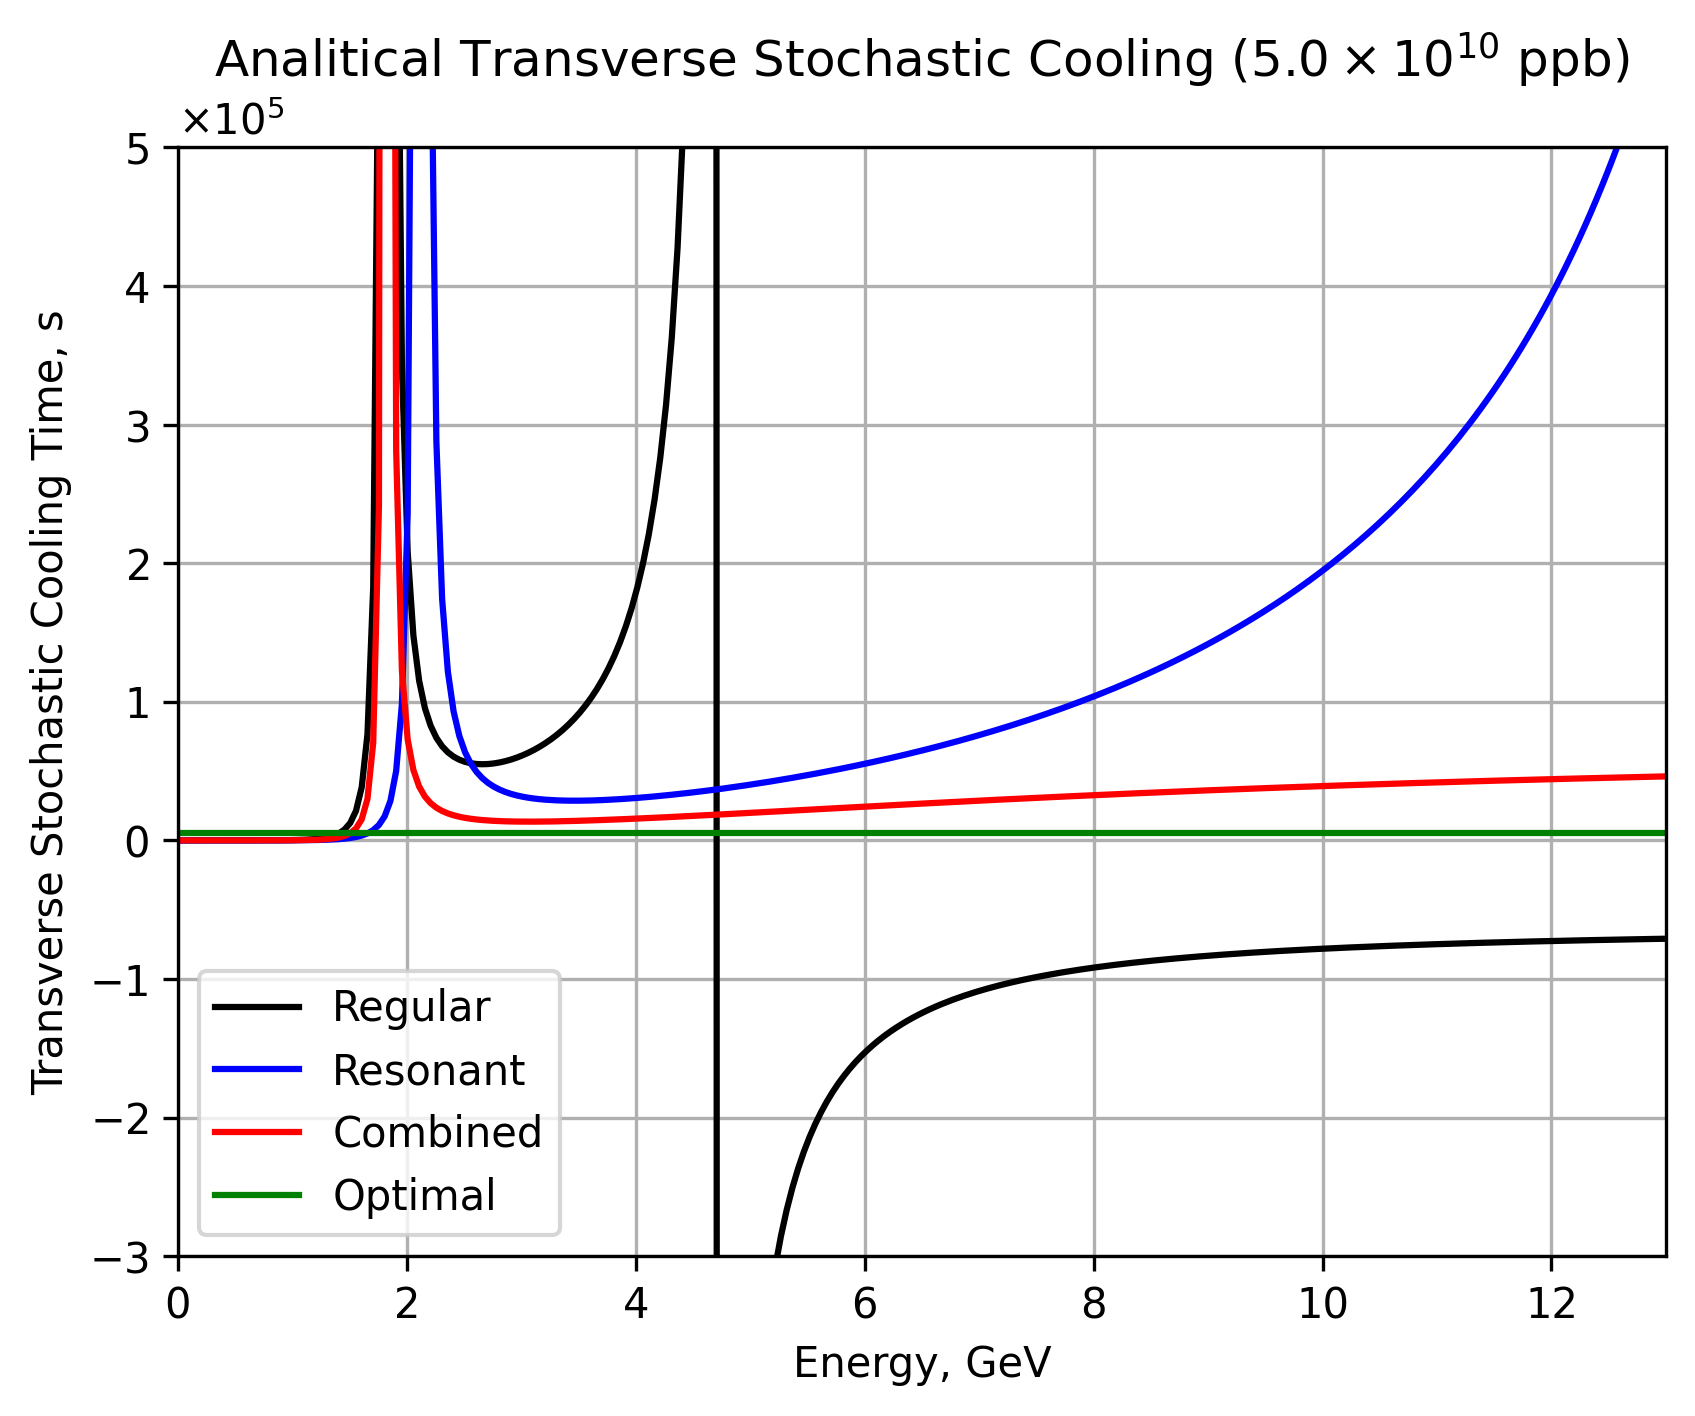
\includegraphics[width=\linewidth]{images/SC_5_0e+10_png}
			\label{fig:sc10e11png}
		\end{minipage}
	\end{figure}
\end{frame}
%------------------------------------------------
\begin{frame}
	\frametitle{Комбинированная структура при пониженной интенсивности}
	\begin{figure}[t]
		\centering
		
\includegraphics[width=8cm]{IBS_SC_5_0e+10_png}
		\label{fig:IBS_SC}
	\end{figure}
\end{frame}